
\chapter{Kibana dashboard}
\label{ch:chapter_three}%
A Kibana dashboard is a data visualization tool commonly used with the Elasticsearch database. It allows users to create interactive, real-time dashboards to analyze and visualize data.

We chose to implement Kibana on the news dataset for two main reasons. Firstly, the technology used for this dataset (Elasticsearch) aligns perfectly with Kibana and its tools. Secondly, Kibana facilitates visual analysis, enabling us to explore and understand our news dataset more comprehensively by identifying patterns and trends through intuitive visualizations.

\newpage

\section{Analysis of key features}
We have analyzed the most important features in order to identify and understand the specific attributes that contribute significantly to the observed patterns and outcomes.

\begin{figure}[h]
  \centering
  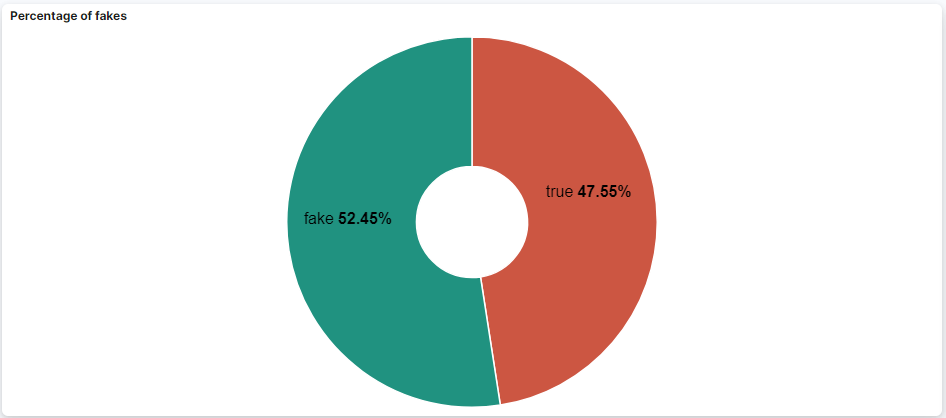
\includegraphics[width=1.0\linewidth]{Images/kibana_1.png}
  \caption{Percentage of fakes and true}
  \label{fig:kibana_1}
\end{figure}

In our dataset, the binary classification feature label distinguishing between fake and non-fake news, exhibits a well-balanced distribution (fig. \ref{fig:kibana_1}). This balance ensures that possible future models of ML are exposed to a representative mix of both classes during training. With approximately equal counts of instances labeled as fake and non-fake, we anticipate that models will be able to learn from a diverse set of examples, contributing to their generalization performance.

\newpage

\begin{figure}[h]
  \centering
  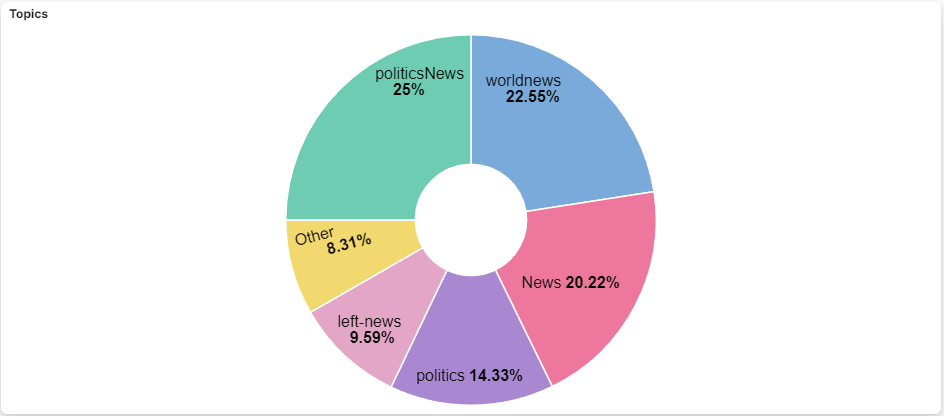
\includegraphics[width=1.0\linewidth]{Images/kibana_2.png}
  \caption{Percentage of topics}
  \label{fig:kibana_2}
\end{figure}

It's important to highlight that the naming conventions for the categories were not consistent between the labels \textbf{fake} and \textbf{true} (fig. \ref{fig:kibana_2}) (i.e. \textit{politicsNews} and \textit{politics} are redundant, or \textit{worldNews} and \textit{News}). This inconsistency in feature naming emphasizes the importance of data preprocessing and standardization to ensure uniformity in our dataset, facilitating accurate model training and evaluation.

For this reason, we have decided to merge \textit{WorldNews} with \textit{GeneralNews} and \textit{Politics News} with \textit{LeftNews} and \textit{Politics}. After this consolidation, the new distribution of categories is as follows:
\begin{itemize}
  \item Merged Politics/Left News: 53.7\%
  \item Merged World/General News: 46.3\%
\end{itemize}

\begin{figure}[h]
  \centering
  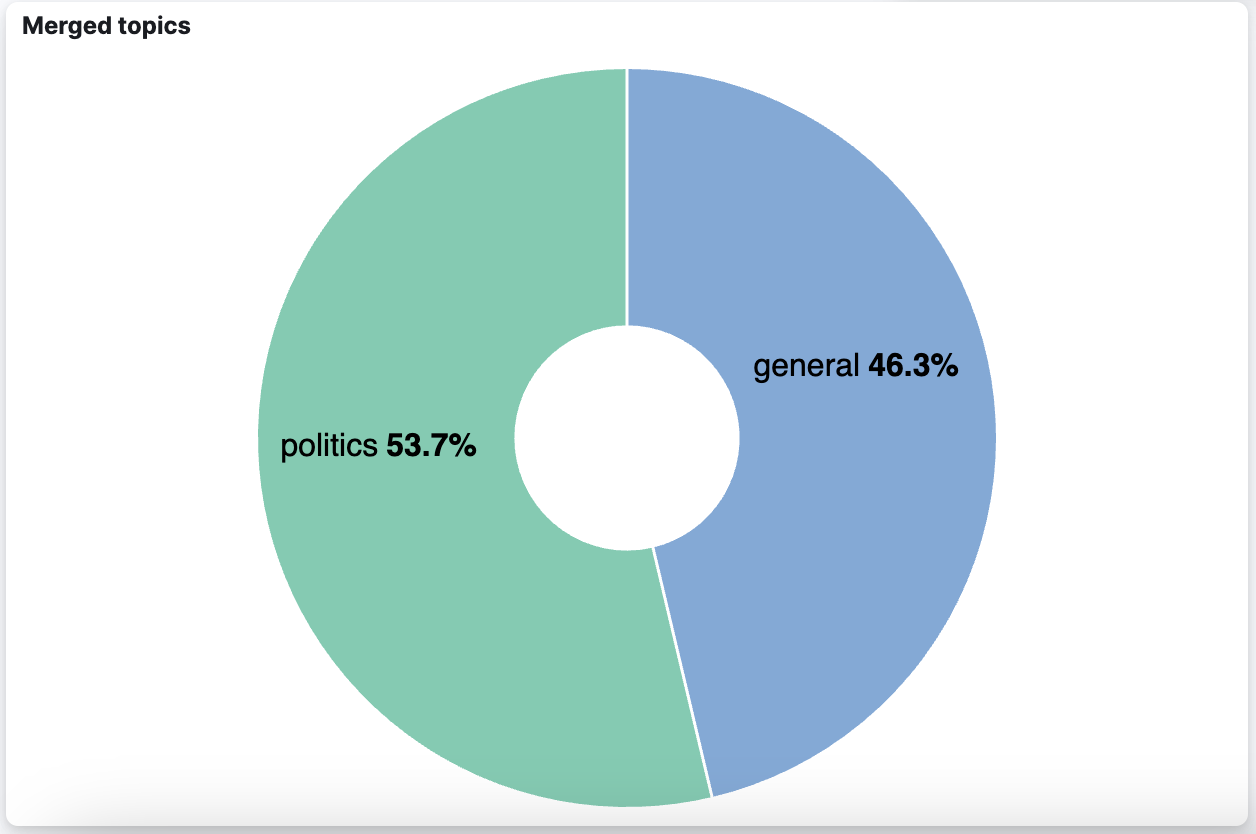
\includegraphics[width=1.0\linewidth]{Images/kibana_6.png}
  \caption{New percentage of topics}
  \label{fig:kibana_6}
\end{figure}

 This dataset covers a range of topics, with a focus on political content represented by the merged \textit{Politics/Left News} category at 53.7\%, and a significant emphasis on global and general news themes within the \textit{Merged World/General News} category, now at 46.3\%.

\newpage


\begin{figure}[h!]
  \centering
  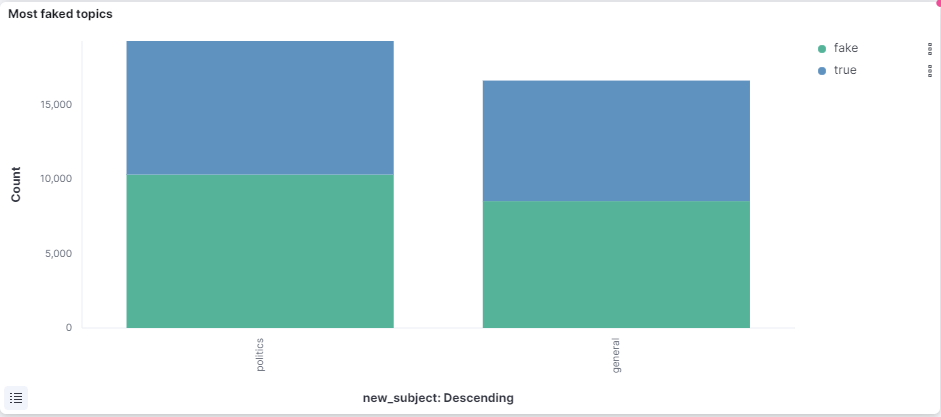
\includegraphics[width=1.1\linewidth]{Images/kibana_4.png}
  \caption{Most faked topics}
  \label{fig:kibana_4}
\end{figure}

Moreover, as expected, each topic is covered by both the \textbf{fake} and \textbf{non-fake} labels, illustrating the comprehensive representation of perspectives across different thematic categories in our dataset.
\\
\\


\begin{figure}[h]
  \centering
  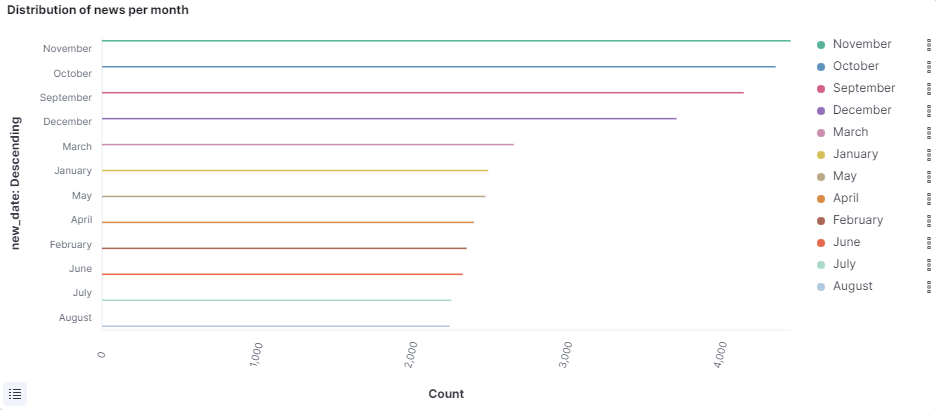
\includegraphics[width=1.0\linewidth]{Images/kibana_3.png}
  \caption{Distribution of news per month}
  \label{fig:kibana_4}
\end{figure}

Another important aspect is the frequency of news articles per month. Analyzing the distribution and trends in the number of news articles over time provides valuable insights into the dataset dynamics.

Overall, winter/fall months are the ones with highest frequency of news in our dataset. In particular, November is the month with most news and August with lowest. 

\newpage

\begin{figure}[h!]
  \centering
  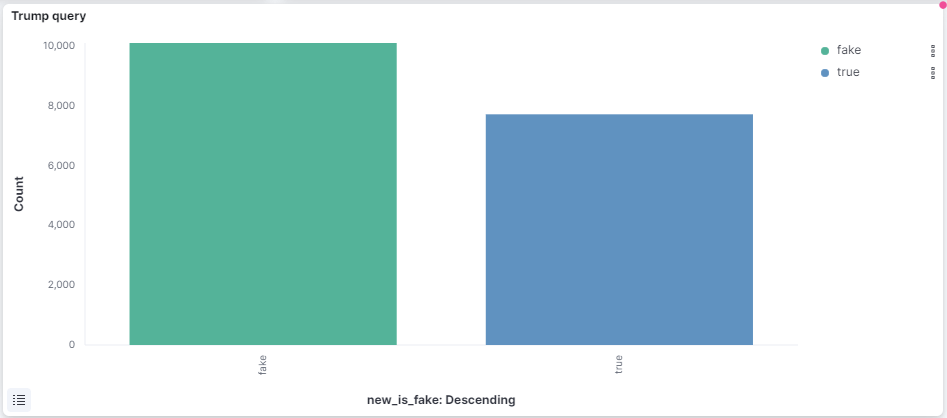
\includegraphics[width=1.0\linewidth]{Images/kibana_5.png}
  \caption{Trump results}
  \label{fig:kibana_4}
\end{figure}

An example of query regarding the difference between fake and true news is about the number of documents that contains the word "Trump".
Overall, there is an abundance of news articles about Trump, indicating a significant presence and emphasis on this topic within our dataset, but in the \textbf{fake} news category, this word is more present than in true news.



\newpage













% LIST OF FIGURES
%\listoffigures

% LIST OF TABLES
%\listoftables

%\cleardoublepage

